\documentclass{cours}
\begin{document}
\setcounter{chapter}{1}
%\shorthandoff{:!}
\chapter{Circuits électriques}
\section{Le courant électrique}
\subsection{Définitions}
Le courant électrique correspond à un déplacement ordonnée de charges électriques. 
\begin{itemize}
\item Les charges peuvent être des particules élémentaires (électrons, protons, ...) ou des entités plus grosse (ions + ou -). La charge est quantifiée, elle est toujours un multiple de $e$ (charge d'un proton)

\item L'origine du courant est aussi variable :
\begin{itemize}
\item Présence d'un champ électrique ;
\item déplacement du milieu dans lequel se trouvent les charges ;
\item charges libres dans le vide.
\end{itemize} 
\end{itemize}

\subsection{Intensité du courant}
L'intensité du courant électrique correspond au \textbf{débit} de la charge électrique à travers une surface $S$.
\begin{center}
  \begin{tikzpicture}[scale=1.4]
    %tikz elec
  \draw (0,0) -- (4,0) ;
  \draw (0,1) -- (4,1) ;
  \draw (2,1) to[bend left=70] (2,0);
   \foreach \x in {1,...,100}
   {
    \pgfmathparse{random()}
    \pgfmathsetmacro\xpos{4*\pgfmathresult}
    \pgfmathparse{random()}
    \pgfmathsetmacro\ypos{\pgfmathresult}
    \fill (\xpos,\ypos) circle (0.02);
   };
  \draw[fill=coul1!30, draw=none,fill opacity=0.5] 
  decorate[decoration={random steps,segment length=2mm}]{(0,0) to[bend left=10] (0,1)}
  --(4,1) 
  decorate[decoration={random steps,segment length=2mm}]{(4,1) to[bend left=10] (4,0)} 
  -- (0,0);
 
  \draw (2,1) to[bend right=70] (2,0);
  \draw[->] (0.5,0.4) -- (1,0.4)  node[midway,above,fill=coul1!15,yshift=0.1cm] {$\vec{v}$};
  \draw[->] (2,-0.25) node[below] {$S$} to[bend right] (2,0.5);
\end{tikzpicture}
\end{center}
On définit l'intensité du courant comme 
\begin{equation*}
I=\frac{Q}{t}
\end{equation*}
avec
\begin{itemize}
\item $Q$ : Quantité de charge qui traverse la surface $S$ (en Coulombs),
\item $t$ : pendant le temps $t$.
\end{itemize}

En faisant tendre le temps $t$ vers 0, on obtient la relation 
\begin{eqencadre}
I=\dfrac{\D Q}{\D t}
\end{eqencadre}

Par exemple, s'il y a $n$ charges $q$ par $\si{m^3}$, avançant à la vitesse $v$, l'intensité du courant est : 

\begin{equation*}
  I=\frac{dQ}{dt} = \frac{nqSvdt}{dt} = \underbrace{nq}_{\rho}Sv
\end{equation*}

$\rho$ est la \emph{densité volumique de charges}

\paragraph{remarques :}
\begin{itemize}
\item L'intensité du courant est une valeur algébrique (il faut définir un sens positif avant de pouvoir la calculer)
\item Pour une même valeur de $I$, les charges + et - se déplacent dans des directions opposées.
\end{itemize}

L'intensité du courant se mesure en Ampères (A) = $\si{C s^{-1}}$. 
\paragraph{Ordres de grandeur :}
\begin{itemize}
\item Dans une montre à quartz : $I\simeq \SI{1}{\micro A}$ ;
\item LED de faible puissance : $I\simeq \SI{10}{mA}$ ;
\item Lampe halogène $I\simeq \SI{1}{A}$ ;
\item foudre $I\simeq \SI{30}{kA}$
\end{itemize}

Nous avons vu que la charge électrique est transportée par des électrons ayant chacun une charge électrique de $-e=\SI{-1.6e-19}{\coulomb}$. On peut donc se demander s'il est bien légitime de parler de courant continu. Prenons par exemple une montre à quartz dans laquelle circule un courant de $i=\SI{1}{\micro\ampere} = \SI{1e-6}{\coulomb\per\second}$. Le nombre d'électrons qui traversent une section du fil à chaque seconde est donc 
\begin{equation}
  n=\frac{\num{1e-6}}{\num{1.6e-19}} \approx \num{6e13}\, \text{electrons/s}
\end{equation}
Le nombre d'électrons qui traversent la section du fil à chaque seconde est tellement élevé qu'il parait légitime de considérer que les électrons forment un flux continu.

\subsection{Régime continu}
En régime continu, l'intensité $I$ du courant, et la densité volumique de charge $\rho$ sont des constantes.

\begin{center}
  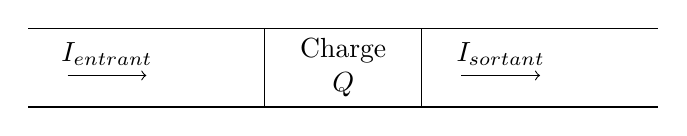
\begin{tikzpicture}
    \draw (0,0) -- (8,0);
    \draw (0,1) -- (8,1);
    \draw (3,0) -- (3,1);
    \draw (5,0) -- (5,1);

    \draw[->] (0.5,0.4) -- (1.5,0.4) node[above,midway] {$I_{\text{entrant}}$};  
    \draw[->] (5.5,0.4) -- (6.5,0.4) node[above,midway] {$I_{\text{sortant}}$};
    \draw (4,0.5) node[align=center] {Charge \\ $Q$};
  \end{tikzpicture}
  \captionof{figure}{Intensité du courant dans une portion de conducteur en régime continu.}
\end{center}

Pendant le temps $dt$ : $dQ=I_{\text{entrant}}\,dt -I_{\text{sortant}}\,dt=(I_{\text{entrant}} -I_{\text{sortant}})\,dt$.

Or $\dfrac{dQ}{dt}=0=I_{\text{entrant}} -I_{\text{sortant}}$. 

Donc $I_{\text{entrant}} =I_{\text{sortant}}$. L'intensité du courant est la même en tout point d'un fil conducteur parcouru par un courant continu.

\subsection{Régime variable}
$I$ est une fonction du temps $I(t)$. On suppose que les variations de $I$ se propagent à la vitesse de la lumière $c$ (en tout cas elles ne peuvent pas aller plus vite)

\begin{center}
  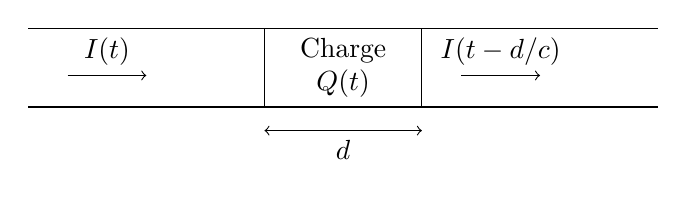
\begin{tikzpicture}
    \draw (0,0) -- (8,0);
    \draw (0,1) -- (8,1);
    \draw (3,0) -- (3,1);
    \draw (5,0) -- (5,1);

    \draw[->] (0.5,0.4) -- (1.5,0.4) node[above,midway] {$I(t)$};  
    \draw[->] (5.5,0.4) -- (6.5,0.4) node[above,midway] {$I(t-d/c)$};
    \draw[<->] (3,-0.3) -- (5,-0.3) node[below,midway] {$d$};
    \draw (4,0.5) node[align=center] {Charge \\ $Q(t)$};
  \end{tikzpicture}
  \captionof{figure}{Intensité du courant dans une portion de conducteur en régime variable.}
\end{center}

Si $I(t)\neq I(t-d/c)$ alors $\dfrac{dQ}{dt} \neq 0$.

\paragraph{Approximation des régimes quasi-stationnaires (ARQS) : } $I$ varie assez lentement pour que $I(t)=I(t-d/c)$. Dans ce cas $\frac{dQ}{dt}=0$ et $I$ est le même en tout point d'un fil conducteur.

Déterminons pour un circuit réel les conditions nécessaires pour pouvoir appliquer l'ARQS :
\begin{itemize}
\item $d$ : dimension du circuit ;
\item $\tau \simeq \dfrac{1}{f}$ : temps typique de variation de $I$ ($f$ est la fréquence typique de variation de $I(t)$).
\end{itemize}
Le temps de propagation d'une variation d'intensité à travers le circuit est $t_I=\dfrac{d}{c}$. Pour être dans les conditions d'application de l'ARQS, il faut que $t_I \ll \tau$, on doit donc avoir :
\begin{loi}{Condition d'application de l'ARQS}
  \begin{equation}
  d\ll \frac{c}{f} \quad \text{ou} \quad df\ll c
  \end{equation}
\end{loi}
L'ARQS est donc applicable à des circuits assez petit pour des fréquences de fonctionnement suffisamment faibles.

\subsection{La loi des n\oe uds}
Dans les conditions de l'ARQS : $\dfrac{dQ}{dt}=0$. On définit un n\oe{}ud  comme la jonction d'au moins 2 fils conducteurs : 
\begin{center}
  \begin{circuitikz}
    \draw (0:2) to[short,i=$i_1$] (0,0);
    \draw (72:2) to[short,i=$i_2$] (0,0);
    \draw (142:2) to[short,i<=$i_3$] (0,0);
    \draw (214:2) to[short,i=$i_4$] (0,0);
    \draw (286:2) to[short,i<=$i_5$] (0,0);
    \draw (0,0) node[circ] {};
    \draw (0,0) circle (0.3) (30:0.3) to[bend left=10] (3,1) node[right] {$Q$};
  \end{circuitikz}
\end{center}
On note $Q$ la charge totale comprise dans le n\oe ud, dans ce cas, on a : $\frac{dQ}{dt}=i_1+i_2-i_3+i_4-i_5=0$. 

\begin{loi}{Loi des n\oe{}uds}
La somme algébrique de tous les courants entrants dans un n\oe{}ud est nulle. 
\begin{equation}
 \sum_{\substack{\text{courants}\\\text{entrants}}}i_k-\sum_{\substack{\text{courants}\\\text{sortants}}}i_k=0
\end{equation}
\end{loi}

\section{La tension électrique}
\subsection{Le potentiel électrique}
Dans un circuit électrique, les charges circulent en perdant de l'énergie potentielle (elles \textit{descendent une pente}). Une charge $q$ possède une énergie potentielle $E_p=qV$ ; $V$ est le \textbf{potentiel électrique} au point considéré. Le potentiel électrique se mesure en Volts (V).

L'origine de l'énergie potentielle est choisie arbitrairement, donc celle de $V$ aussi. Le point du circuit où $V$ est choisi nul est \textbf{la référence de potentiel}.

\subsection{La tension électrique}
La tension électrique $U_{AB}$ entre deux points $A$ et $B$ d'un circuit est la différence de potentiel entre ces deux points :

\begin{center}
  \begin{circuitikz}[european]
    \draw (0,0) node[below left] {A} to[R,*-*] (3,0) node[below right] {B};
    \draw[dotted] (3,0) to[R] (6,0);
    \draw[dotted] (0,0) to[R] (-3,0);
    \draw[<-] (0,0.5) -- (3,0.5) node[midway,above]{$U_{AB}=V_A-V_B$}; 
    \draw[->] (0,-0.5) -- (3,-0.5) node[midway,below]{$U_{BA}=V_B-V_A$}; 
  \end{circuitikz}
\end{center}

\paragraph{Remarques :}
\begin{itemize}
\item La tension est une grandeur algébrique : $U_{BA}=V_B-V_A=-U_{AB}$
\item La tension se mesure en Volts (V) (d'après Alessandro Volta (1745--1827) qui a inventé la première pile électrique)
\end{itemize}

\paragraph{Ordres de grandeur :}
\begin{itemize}
\item Petits appareils électroniques $\simeq \SI{5}{V}$ ;
\item électroménager $\simeq \SI{220}{V}$ ;
\item lignes haute-tension $\simeq \SI{400}{kV}$ ;
\item foudre $\simeq \SI{e8}{V}$.
\end{itemize}

\subsection{La loi des mailles}
Une \textbf{maille} est une portion de circuit formant une boucle fermée :
\begin{center}
  \begin{circuitikz}[european,scale=0.7]
    %tikz elec
    \draw (0,0) node[above left] {A} to[R,*-*] (3,0) node[above left] {B} to[R,*-*] (6,0) node[above right] {C} to[R,*-*] (6,-3) node[below right] {D} to[R,*-*] (3,-3) node[below]{E} to[R,*-] (0,-3) to[short] (0,0); 

   \draw[dotted] (3,-3) to[R] (3,0);
   \draw[dotted] (6,-3) to[R] (9,-3);
   \draw[dotted] (6,0) to[R] (9,0);

   \draw[<-] (0.1,0.7) -- (2.9,0.7) node[midway,above] {$U_{AB}$};
   \draw[<-] (3.1,0.7) -- (5.9,0.7) node[midway,above] {$U_{BC}$};
   \draw[<-] (6.7,-0.1) -- (6.7,-2.9) node[midway,right] {$U_{CD}$};
   \draw[->] (3.1,-3.7) -- (5.9,-3.7) node[midway,below] {$U_{DE}$};
   \draw[->] (0.1,-3.7) -- (2.9,-3.7) node[midway,below] {$U_{EA}$};
  \end{circuitikz}
\end{center}

On a : $U_{AB}+U_{BC}+U_{CD}+U_{DE}+U_{EA}=V_A-V_B+V_B-V_C+\ldots+V_E-V_A=0$. 

\begin{loi}{Loi des mailles}
  La somme des tensions (orientées dans le même sens de rotation) d'une maille est nulle.
\end{loi}

\noindent La loi des n\oe{}uds et la loi des mailles constituent les \textbf{lois de Kirchoff}.

\section{Le dipôle électrique}
\subsection{Définition}
Un dipôle est un composant qui comporte 2 bornes.
\begin{center}
  \begin{circuitikz}[european]
    \draw (0,0) node[below left] {A} to[R,*-*,i>_=$i_{AB}$] (3,0) node[below right] {B};
    \draw[<-] (0,0.5) -- (3,0.5) node[midway,above]{$U_{AB}$};
  \end{circuitikz}
\end{center}

\subsection{Puissance reçue}
Le puissance électrique \textbf{reçue} par le dipôle $AB$ est :
\begin{eqencadre}
P = U_{AB}\times i_{AB}
\end{eqencadre}
La puissance se mesure en Watts (W=J/s), d'après le physicien écossais James \textsc{WATT} (1736--1819).

\paragraph{Remarque : } Si le dipôle produit de l'énergie, $P<0$.

\subsection{Convention récepteur ou générateur}
Un récepteur convertit l'énergie électrique qu'il reçoit en une autre forme d'énergie (mécanique, thermique). On a $P_{\text{reçue}}>0$ donc $u$ et $i$ ont des sens opposés (\textbf{convention récepteur})
\begin{center}
  \begin{circuitikz}[european]
    \draw (0,0) node[left] {A} to[R,*-*,i>_=$i_{AB}>0$] (4,0) node[right] {B};
    \draw[<-] (0,0.5) -- (4,0.5) node[midway,above]{$U_{AB}>0$};
  \end{circuitikz}
\end{center}

Un générateur fournit de l'énergie électrique donc $P_{\text{reçue}}<0$, $u$ et $i$ sont dans le même sens (\textbf{convention générateur})
\begin{center}
  \begin{circuitikz}[european]
    \draw (0,0) node[left] {A} to[R,*-*,i>_=$i_{AB}>0$] (4,0) node[right] {B};
    \draw[->] (0,0.5) -- (4,0.5) node[midway,above]{$U_{BA}>0$};
  \end{circuitikz}
\end{center}

\subsection{Caractéristique d'un dipôle}
Dans un dipôle il existe une relation entre la tension $u$ à ses bornes et l'intensité $i$ qui le traverse. On peut parfois mettre cette relation sous la forme $u=f(i)$ ou $i=g(u)$. Cette relation entre $u$ et $i$ est la \textbf{caractéristique statique du dipôle}.
\begin{center}
  \begin{tikzpicture}[scale=0.7]
    \draw[->] (-3,0) -- (3,0) node[right] {$i$};
    \draw[->] (0,-2) -- (0,2) node[above] {$u$};
    \draw[coul1] plot[smooth,tension=1] coordinates {(-3,-2) (-2,-0.5) (0,0) (2,0.7) (3,1.8)} node[above right] {$u=f(i)$};
  \end{tikzpicture}
  \captionof{figure}{Courbe représentative de la caractéristique statique tension-courant d'un dipôle.}
\end{center}

\paragraph{Remarques :}
\begin{itemize}
\item Si la caractéristique passe par $(0,0)$, c'est un dipôle \textbf{passif}, sinon il est \textbf{actif}.
\item Si c'est une droite, on dit que le dipôle est \textbf{linéaire}.
\item Le point de la caractéristique où se trouve le dipôle (sa tension et son intensité) est le \textbf{point de fonctionnement}
\end{itemize}


\section{Le dipôle résistance}
\subsection{Généralités}
Symbole : 
\tikz[baseline=-0.25em,scale=0.7]{\draw[european] (0,0) to[R] (3,0);} (ou \tikz[baseline=-0.25em,scale=0.7]{\draw[american] (0,0) to[R] (3,0);})

On utilise la convention récepteur : 
  \begin{circuitikz}[european,scale=0.7,baseline=-0.25em]
    \draw (0,0) node[left] {A} to[R,*-*,i>_=$i$] (3,0) node[right] {B};
    \draw[<-] (0,0.5) -- (3,0.5) node[midway,above]{$u$};
  \end{circuitikz}

La caractéristique d'une résistance est 
\begin{eqencadre}
u=Ri
\end{eqencadre}
c'est la \textbf{loi d'Ohm}. $R$ est la valeur (résistance) du dipôle en Ohm ($\Omega$) (Georg Simon Ohm 1789--1854)

On définit aussi la conductance $G=\dfrac{1}{R}$ en $\si{\ohm^{-1}}$ ou Siemens (S).

\paragraph{fabrication : } On utilise un matériau de résistivité $\rho$ de longueur $L$ et de section $S$ :
\begin{center}
  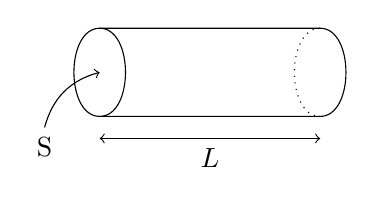
\begin{tikzpicture}[scale=1.4]
    \draw (0,0.4) to[bend left=90] (0,-0.4) to[bend left=90] (0,0.4);
    \draw (0,0.4) -- (2,0.4) to[bend left=90] (2,-0.4) -- (0,-0.4);
    \draw[dotted] (2,0.4) to[bend right=90] (2,-0.4);
    \draw[->] (-0.5,-0.5) node[below] {S} to[bend left] (0,0);
    \draw[<->] (0,-0.6) -- (2,-0.6) node[midway,below] {$L$};
  \end{tikzpicture}
\end{center}
La résistance de ce conducteur est $R=\dfrac{\rho L}{S}$.

\subsection{Effet Joule}
Une résistance convertit l'intégralité de la puissance électrique reçue en chaleur (effet Joule)

\begin{circuitikz}[european,scale=0.7,baseline=-0.25em]
  \draw (0,0) node[left] {A} to[R,*-*,i>_=$i$] (3,0) node[right] {B};
  \draw[<-] (0,0.5) -- (3,0.5) node[midway,above]{$u$};
\end{circuitikz}
$P_{\text{reçue}}=u\cdot i=Ri\cdot i$ donc 
\begin{loi}{Puissance reçue par effet Joule par une résistance}
 \begin{equation}
   P_{\text{reçue}} = Ri^2 = \frac{u^2}{R}
 \end{equation} 
\end{loi}


\paragraph{Remarque :}L'énergie reçue par la résistance entre les instants $t_1$ et $t_2$ est : $E=\displaystyle\int_{t_1}^{t_2}P(t)\,\D{}t=\int_{t_1}^{t_2}Ri(t)^{2}\,\D{}t$

\subsection{Association de résistances}
\paragraph{En série : } 
\begin{circuitikz}[european,scale=1,baseline=-0.25em]
  \draw (0,0) node[above] {A} to[R=$R_1$,*-*,i>_=$i$] (3,0) node[above] {B} to[R=$R_2$,*-*,i_=$i$] (6,0) node[above] {C};
  \draw[<-] (0.5,-0.5) -- (2.5,-0.5) node[midway,below]{$U_1$};
  \draw[<-] (3.5,-0.5) -- (5.5,-0.5) node[midway,below]{$U_2$};
  \draw[<-] (0.5,-1) -- (5.5,-1) node[midway,below]{$U_{AC}$};
\end{circuitikz}
\hspace{1cm}Circuit équivalent : 
\begin{circuitikz}[european,scale=0.7,baseline=-0.25em]
  \draw (0,0) node[left] {A} to[R=$R_{eq}$,*-*,i>^=$i$] (3,0) node[right] {C};
  \draw[<-] (0,-0.5) -- (3,-0.5) node[midway,below]{$U_{AC}$};
\end{circuitikz}

La loi des mailles donne : $U_1+U_2-U_{AC}=0$ donc $U_{AC}=U_1+U_2$. D'après la loi d'Ohm, on a $U_1=R_1i$ et $U_2=R_2i$. D'où finalement $U_{AC}=R_1i+R_2i=(R_1+R_2)i$.

La résistance équivalente à deux résistance branchées en série est : \res{$R_{eq}=R_1+R_2$}

On généralise se résultat à $n$ résistances $R_1,R_2,\dots,R_n$ branchées en série : 
\begin{eqencadre}
  R_{eq}=\displaystyle\sum_{i=1}^nR_i
\end{eqencadre}

\begin{application}
Pont diviseur de tension : 
\begin{circuitikz}[european,scale=1,baseline=-0.25em]
  \draw (0,0) node[above] {A} to[R=$R_1$,*-*,i>_=$i$] (3,0) node[above] {B} to[R=$R_2$,*-*,i_=$i$] (6,0) node[above] {C};
  \draw[<-] (0.5,-0.5) -- (2.5,-0.5) node[midway,below]{$U_1$};
  \draw[<-] (3.5,-0.5) -- (5.5,-0.5) node[midway,below]{$U_2$};
  \draw[<-] (0.5,-1) -- (5.5,-1) node[midway,below]{$U_{AC}$};
\end{circuitikz}

$U_{AC}=R_{eq}i$ donc $i=\dfrac{U_{AC}}{R_{eq}}$.

$U_2=R_2i=\dfrac{R_2}{R_{eq}}U_{AC}$ donc finalement \res{$U_2=\dfrac{R_2}{R_1+R_2}U_{AC}<U_{AC}$}
\end{application}

\paragraph{En parallèle :}
\begin{circuitikz}[european,baseline=-0.25em]
\draw (0,0) to[short,i=$i$,-*] (1,0) node[above left] {A} to[short] (1,0.5) to[R=$R_1$,i=$i_1$] (3,0.5) to[short,-*] (3,0) node[above right] {$B$} to[short] (4,0);
\draw (1,0) to[short] (1,-0.5) to[R,l=$R_2$,i=$i_2$] (3,-0.5) to[short,-*] (3,0);
\draw[<-] (1,-1) -- (3,-1) node[midway,below] {$U_{AB}$};
\end{circuitikz}
\hspace{1cm}Circuit équivalent : 
\begin{circuitikz}[european,scale=0.7,baseline=-0.25em]
  \draw (0,0) node[left] {A} to[R=$R_{eq}$,*-*,i>^=$i$] (3,0) node[right] {B};
  \draw[<-] (0,-0.5) -- (3,-0.5) node[midway,below]{$U_{AB}$};
\end{circuitikz}

Loi des n\oe{}uds : $i=i_1+i_1 = \dfrac{U_{AB}}{R_1}+\dfrac{U_{AB}}{R_2}=U_{AB}\left( \dfrac{1}{R_1} + \dfrac{1}{R_2} \right) = \dfrac{U_{AB}}{R_{eq}}$

Deux résistances $R_1$ et $R_2$ branchées en parallèle sont équivalentes à une résistance $R_{eq}$ de valeur : $\dfrac{1}{R_{eq}}=\dfrac{1}{R_1}+\dfrac{1}{R_2}$

La conductance équivalente est $G_{eq}=G_1+G_2$.

On généralise se résultat à $n$ résistances $R_1,R_2,\dots,R_n$ branchées en parallèle : 
\begin{eqencadre}
  \frac{1}{R_\text{eq}}=\sum_{i=1}^n \frac{1}{R_i} \quad \text{ou} \quad G_{eq}=\sum_{i=1}^nG_i
\end{eqencadre}

\begin{application}
Pont diviseur de courant :
\begin{center}
\begin{circuitikz}[european,baseline=-0.25em]
\draw (0,0) to[short,i=$i$,-*] (1,0) node[above left] {A} to[short] (1,0.5) to[R=$R_1$,i=$i_1$] (3,0.5) to[short,-*] (3,0) node[above right] {$B$} to[short] (4,0);
\draw (1,0) to[short] (1,-0.5) to[R,l=$R_2$,i=$i_2$] (3,-0.5) to[short,-*] (3,0);
\draw[<-] (1,-1) -- (3,-1) node[midway,below] {$U_{AB}$};
\end{circuitikz}
\end{center}

\begin{equation}
  i=G_\text{eq} U_{AB} \quad \text{et} \quad i_1=G_1 U_{AB} \quad \text{soit} \quad i_1=\frac{G_1}{G_1+G_2}i<i
\end{equation}
\end{application}
 

\section{Le condensateur}
\subsection{Généralités}
Un condensateur est un dipôle formé par 2 armatures métaliques séparées par un matériau isolant. 

Symbole :~%
\begin{circuitikz}[baseline=-0.25em]
  \draw (0,0) to[C,i>^=$i$] (3,0);
  \draw[<-] (0,-0.5) -- (3,-0.5) node[midway,below] {$u$};
  \draw (1,0.5) node {$+q$};
  \draw (2,0.5) node {$-q$};
\end{circuitikz}

Les armatures stockent des charges électriques. En régime continu, $i=0$ (le condensateur se comporte comme un isolant).

En régime variable, $i=\dfrac{\D q}{\D t}$ et $q=Cu$, donc 

\begin{eqencadre}
  i=C\frac{\D u}{\D t}
\end{eqencadre}

$C$ est une constante, c'est la \textbf{capacité} du condensateur, on la mesure en farad (\si{F}=$\si{A\,s\,V^{-1}}$=$\si{s\,\ohm^{-1}}$)

\paragraph{remarque : } $u(t_2)-u(t_1) = \displaystyle \int_{t_1}^{t_2}\frac{i(t)}{C}\,\D t$, à la limite où $t_1\rightarrow t_2$, on a $u(t_1)=u(t_2)$ donc la tension est continue aux bornes d'un condensateur.

\subsection{\'Energie stockée}
 \begin{circuitikz}[baseline=-0.25em]
  \draw (0,0) to[C,i>^=$i$] (3,0);
  \draw[<-] (0,-0.5) -- (3,-0.5) node[midway,below] {$u$};
\end{circuitikz}
La puissance reçue est $P_{\text{reçue}}=u\cdot i=u\cdot C\dfrac{\D u}{\D t}=\dfrac{1}{2}C \dfrac{\D (u^2)}{\D t}$. 

Donc l'énergie stockée dans le condensateur est : $E=\displaystyle\int_{t=0}^T \frac{1}{2}C \frac{\D (u^2)}{\D t}\, \D t$, soit 
\begin{eqencadre}
  \displaystyle E=\frac{1}{2}Cu^2 \quad \text{en joules}
\end{eqencadre}

L'énergie est stockée dans le champ électrique créé entre les armatures.

\section{La bobine}
\subsection{Généralités}
C'est un dipôle formé par l'enroulement d'un fil conducteur.

Symbole :%
\begin{circuitikz}[baseline=-0.25em]
  \draw (0,0) to[L,i>^=$i$] (3,0);
  \draw[<-] (0,-0.5) -- (3,-0.5) node[midway,below] {$u$};
\end{circuitikz}

En régime continu, $u=0$ car c'est un fil conducteur.

En régime variable : 

\begin{eqencadre}
  u(t)=L \dfrac{\D i}{\D t}
\end{eqencadre}
$L$ est \textbf{l'inductance} de la bobine en henry (\SI{1}{\henry}=$\SI{1}{\volt\second\per\ampere}$).

\paragraph{remarque :} $i(t_2) = i(t_1)+\displaystyle \frac{1}{L}\int_{t_1}^{t_2}u(t)\,\D t$ donc l'intensité $i(t)$ est continue dans une bobine.

\subsection{\'Energie stockée}
\begin{circuitikz}[baseline=-0.25em]
  \draw (0,0) to[L,i>^=$i$] (3,0);
  \draw[<-] (0,-0.5) -- (3,-0.5) node[midway,below] {$u$};
\end{circuitikz}
La puissance reçue est $P_{reçue}=u\cdot i = L \dfrac{\D i}{\D t}=L \dfrac{\D (i^2)}{\D t}$. 

Donc l'énergie stockée dans la bobine est : $E = \displaystyle\int_{t=0}^T \frac{1}{2}L \frac{\D (i^2)}{\D t}\, \D t$, soit 
\begin{eqencadre}
  E=\frac{1}{2}Li^2 \quad \text{en joules}
\end{eqencadre}

L'énergie est stockée dans le champ magnétique créé par la bobine.

\section{Générateurs}
\subsection{Source de tension}
Une source idéale de tension est un dipôle électrique dont la tension aux bornes ne dépend pas de l'intensité du courant qui le traverse.

Symbole : %
\begin{circuitikz}[baseline=-0.25em]
  \draw (0,0) to[V,v=$E$, i=$i$] (3,0);
  \draw[->] (0,-0.5) -- (3,-0.5) node[midway,below] {$u$};
\end{circuitikz} %
\hspace{2cm}
Caractéristique : %
\begin{tikzpicture}[scale=0.5,baseline=-0.25em]
  \draw[->] (-1,0) -- (4,0) node[below] {$u$};
  \draw[->] (0,-2) -- (0,2) node[left] {$i$};
  \draw[coul1] (2,-2) -- (2,2);
  \draw (2,0) node[below right] {$E$};
\end{tikzpicture}

Une source de tension non idéale (modèle linéaire) est modélisée par : %
\begin{circuitikz}[baseline=-0.25em,european]
  \draw (0,0) to[V,v=$E$, i=$i$] (2,0) to[R,l=$R$] (4,0);
  \draw[->] (0,-0.5) -- (4,-0.5) node[midway,below] {$u$};
  \draw[->] (4,0.7) -- (2,0.7) node[midway,above] {$u_R$}; 
\end{circuitikz} %

$E$ est la force électromotrice (fém) de la source de tension, et $R$ sa résistance interne.

$u=E-u_R=E-Ri$, ce qui donne la caractéristique : %
\begin{tikzpicture}[scale=0.5,baseline=-0.25em]
  \draw[->] (-1,0) -- (4,0) node[below] {$u$};
  \draw[->] (0,-2) -- (0,2) node[left] {$i$};
  \draw[coul1] (-1,1.5) -- (4,-1);
  \draw (2,0) node[below left] {$E$};
  \draw (2,3pt) -- (2,-3pt);
  \draw[->] (2,1) node[right] {pente : $-\frac{1}{R}$} to[bend right] (1,0.5);
\end{tikzpicture}

\subsection{Source de courant}
Une source idéale de courant est un dipôle parcouru par un courant constant quelle que soit la tension à ses bornes.

Symbole : %
\begin{circuitikz}[baseline=-0.25em]
  \draw (0,0) to[I=$I_0$] (3,0);
  \draw (2.5,0.3) node {$i$};
  \draw[->] (0,-0.5) -- (3,-0.5) node[midway,below] {$u$};
\end{circuitikz} %
\hspace{2cm}
Caractéristique : %
\begin{tikzpicture}[scale=0.5,baseline=-0.25em]
  \draw[->] (-1,0) -- (4,0) node[below] {$u$};
  \draw[->] (0,-2) -- (0,2) node[left] {$i$};
  \draw[coul1] (-1,1) -- (4,1);
  \draw (0,1) node[above right] {$I_{0}$};
\end{tikzpicture}

Une source de courant non idéale (modèle linéaire) est modélisée par : %
\begin{tikzpicture}[european,baseline=-0.25em]
  \draw (0,0) to[short] (1,0) to[short] (1,0.5) to[I=$I_0$] (3,0.5) to[short] (3,0) to[short,i=$i$] (4,0);
  \draw (1,0) to[short] (1,-0.5) to[R,l_=$R$,i<=$i_r$] (3,-0.5) to[short] (3,0);
  \draw[->] (0,-1.2) -- (4,-1.2) node[midway,below] {$u$};
\end{tikzpicture}

$i=I_0-i_R=I_0-\dfrac{u}{R}$, ce qui donne la caractéristique :
\begin{tikzpicture}[scale=0.5,baseline=-0.25em]
  \draw[->] (-1,0) -- (4,0) node[below] {$u$};
  \draw[->] (0,-2) -- (0,2) node[left] {$i$};
  \draw[coul1] (-1,1.5) -- (4,-1);
  \draw (0,1) node[above right] {$I_0$};
  \draw (-3pt,1) -- (3pt,1);
  \draw[->] (2,1) node[right] {pente : $-\frac{1}{R}$} to[bend right] (1,0.5);
\end{tikzpicture}

\subsection{\'Equivalence entre sources non idéales linéaires}

On considère la source de courant non idéale suivante :
%
%\begin{center}
  \begin{tikzpicture}[european,baseline=-0.25em]
  \draw (0,0) to[short] (1,0) to[short] (1,0.5) to[I=$I_0$] (3,0.5) to[short] (3,0) to[short,i=$i$] (4,0);
  \draw (1,0) to[short] (1,-0.5) to[R,l_=$R$,i<=$i_r$] (3,-0.5) to[short] (3,0);
  \draw[->] (0,-1.2) -- (4,-1.2) node[midway,below] {$u$};
\end{tikzpicture} 
\hspace{1cm}(représentation de Norton)
%\end{center}

$i=I_0-i_R=I_0-\dfrac{u}{R} \Rightarrow u=\underbrace{RI_0}_E-Ri$ qui est la caractéristique d'une source de tension non idéale de fém $E=RI_0$ et de résistance interne $R$ :

\begin{center}
  \begin{circuitikz}[baseline=-0.25em,european]
  \draw (0,0) to[V,v=\mbox{$E=RI_0$}, i=$i$] (2,0) to[R,l=$R$] (4,0);
  \draw[->] (0,-0.5) -- (4,-0.5) node[midway,below] {$u$};
\end{circuitikz} 
\hspace{2cm}(représentation de Thévenin)
\end{center}

\end{document}

%%% Local Variables: 
%%% mode: latex
%%% LaTeX-command: "latex -shell-escape"
%%% End: 
